\documentclass{article}

\usepackage[margin=0.5in]{geometry}
\usepackage{graphicx}

\title{1.1 Systems of Equations Homework}
\author{}
\date{}

\begin{document}
\maketitle
\begin{enumerate}
    \item The sum of two numbers is $20$ and their difference is $5$.
        What is the smaller of the two numbers?
        \vspace{3cm}
    \item On a certain standardized test with $50$ problems, $5$ points were awarded for each correct answer, and $1$ point was deducted for each incorrect answer.
        Chloe answered all the questions on the test and scored a total of $184$ points.
        How many questions did she answer correctly?
        \vspace{3cm}
    \item Rectangles $R_1$ and $R_2$, and squares $S_1$, $S_2$, and $S_3$, shown below, combine to form a rectangle that is $3322$ uints wide and $2020$ units high.
        What is the side length of $S_2$ in units?
        \begin{center}
            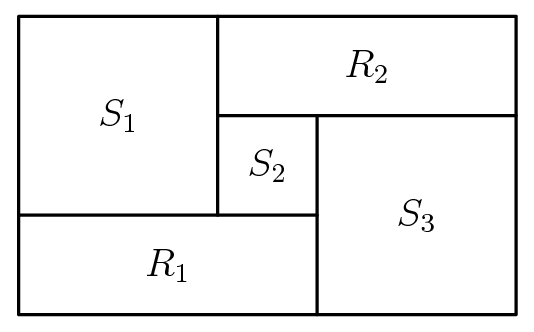
\includegraphics[scale=0.2]{1-1rectangles.png}
        \end{center}
        \vspace{3cm}
    \item Each of the points $A$, $B$, $C$, $D$, $E$, and $F$ in the figure below represent a different digit from $1$ to $6$.
        Each of the five lines shown passes through some of these points.
        The digits along each line are added to produce five sums, one for each line.
        The total of the five sums is $47$.
        What is the digit represented by $B$?
        \begin{center}
            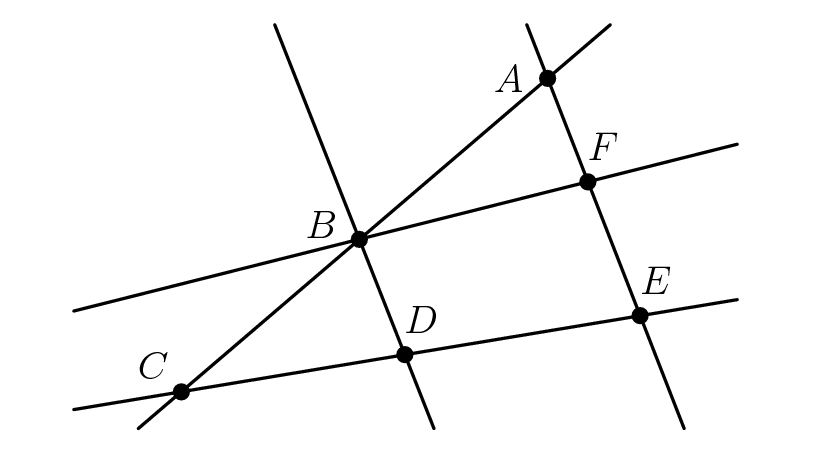
\includegraphics[scale=0.2]{1-1lines.png}
        \end{center}
\end{enumerate}
\end{document}
